\documentclass{beamer}
\setbeameroption{hide notes}
\usepackage{graphicx}
\usepackage[abspath]{currfile}
\usepackage{ifthen, pdftexcmds}

\newcommand*{\dir}{.}

\makeatletter
\ifnum\pdf@strcmp{\currfilepath}{TemplateSlides.tex}=0
	\renewcommand*{\dir}{./../..}
\fi
\makeatother

\AtBeginSection[]{
\begin{frame}
	\begin{beamercolorbox}[center]{title}
	\usebeamerfont{title}\insertsectionhead
	\end{beamercolorbox}
\end{frame}
}

\title{Presentation title}
\author{Author}
\institute{Affiliation}
\date{\today}

\begin{document}

\frame{\titlepage}

\section{Section}

\begin{frame}
\frametitle{Research question}
\begin{itemize}
	\item Point One 
	\note{Notes on Main point}
	\begin{itemize}
		\item Sub Point
		\item Sub Point  
		\note{Notes on subpoint}
	\end{itemize}
 	\item Point Two
\end{itemize}
\end{frame}

\begin{frame}
\frametitle{Results}
\begin{centering}
\medskip{}
\par\end{centering}
\begin{centering}
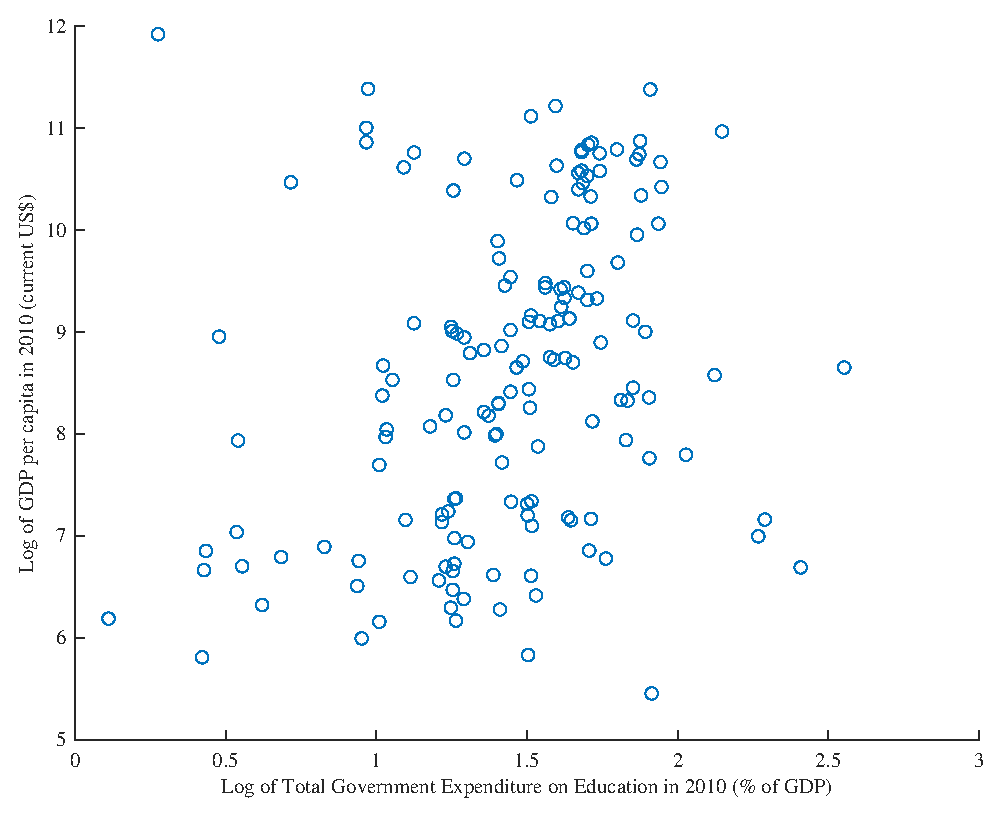
\includegraphics[width=0.7\linewidth]{\dir/output/analysis/plots/gdp_educ}\medskip{}
\par\end{centering}
\end{frame}

\end{document}
